\chapter{Processi Primari}\label{ProcessiPrimari}
\section{Fornitura}\label{ProcessiPrimariFornitura}

\subsection{Scopo}\label{ProcessiPrimariFornituraScopo}
La fornitura secondo lo standard ISO/IEC 12207:1995 descrive le attività$_G$ e i compiti svolti dal fornitore al fine di sviluppare un prodotto soddisfacente e che rispetti appieno le richieste del committente$_G$.
Durante questa fase si prevede la compilazione di diversi documenti, i quali verranno inviati al committente$_{\scaleto{G}{3pt}}$ per guadagnare la possibilità di lavorare al progetto offerto dall'azienda \textit{Sync Lab}.
Il fornitore esegue un'attività$_{\scaleto{G}{3pt}}$ di analisi e stesura dello \textit{Studio di Fattibilità}, documento che rileva i rischi e le criticità riscontrate nella richiesta di appalto.
Si definisce inoltre un accordo contrattuale con il proponente$_G$ mediante il quale si regolano i rapporti con l'azienda, la consegna e la manutenzione del prodotto sviluppato.

\subsection{Descrizione}\label{ProcessiPrimariFornituraDescrizione}
Nella seguente sezione sono contenute tutte le norme che ogni componente del gruppo deve seguire per essere i fornitori$_G$ del proponente$_{\scaleto{G}{3pt}}$ \textit{Sync Lab} e del committente$_{\scaleto{G}{3pt}}$ \textit{Prof. Tullio Vardanega}.

\subsection{Aspettative}\label{ProcessiPrimariFornituraAspettative}
Il gruppo si aspetta di instaurare e mantenere un costante rapporto collaborativo con l'azienda \textit{Sync Lab} ed in particolare con il referente \textit{Fabio Pallaro}.

\subsection{Studio di Fattibilità}\label{ProcessiPrimariFornituraStudioDiFattibilità}
Lo \textit{Studio di Fattibilità} consiste nell'analisi e nella valutazione sistematica delle caratteristiche, dei costi, e dei possibili risultati di un progetto sulla base di una preliminare idea di massima.
A seguito della presentazione dei capitolati d'appalto da parte di ogni proponente$_{\scaleto{G}{3pt}}$ avvenuta il 2020-11-05, il \textit{Responsabile di Progetto} si è impegnato a programmare incontri con tutti i componenti del gruppo \textit{Jawa Druids} per valutare le scelte di ogni membro e attuare così un primo scambio di idee. Una volta individuato il capitolato d'interesse gli \textit{Analisti} hanno provveduto alla stesura dello \textit{Studio di Fattibilità}, i quali hanno fornito un'analisi accurata dei capitolati presentati.
Nella stesura dello \textit{Studio di Fattibilità} per ogni capitolato$_{\scaleto{G}{3pt}}$ si riporterà:
\begin{itemize}
	\item informazioni generali: informazioni riguardanti il proponente$_{\scaleto{G}{3pt}}$;
	\item descrizione del capitolato$_{\scaleto{G}{3pt}}$: sintesi del progetto da sviluppare;
	\item finalità del progetto: finalità richieste dal capitolato$_{\scaleto{G}{3pt}}$ d'appalto;
	\item tecnologie interessate: tecnologie che verranno utilizzate nello svolgimento del capitolato$_{\scaleto{G}{3pt}}$;
	\item aspetti positivi: aspetti favorevoli alla scelta del capitolato$_{\scaleto{G}{3pt}}$;
	\item criticità e fattori di rischio: problematiche che potrebbero sorgere durante lo svolgimento del capitolato;
	\item conclusioni: accettazione o rifiuto del capitolato$_{\scaleto{G}{3pt}}$ in base alle informazioni illustrate precedentemente e anche all'interesse dimostrato da ogni membro nel gruppo.
\end{itemize}
\subsection{Altra documentazione da fornire}\label{ProcessiPrimariFornituraAltraDocumentazioneDaFornire}
Oltre allo \textit{Studio di Fattibilità} vengono consegnati altri documenti all'azienda \textit{Sync Lab} ed ai committenti \textit{Prof. Tullio Vardanega} e \textit{Prof. Riccardo Cardin}. Questi documenti sono necessari al fine di tracciare le attività$_{\scaleto{G}{3pt}}$ di Analisi, Pianificazione, Verifica, Validazione e Controllo di Qualità per assicurare una completa trasparenza durante tutta la durata del ciclo di vita del progetto.
I documenti in questione sono:
\begin{itemize}
	\item \textit{Analisi dei Requisiti 4.0.0}: identifica e dettaglia in modo completo ed esaustivo i requisiti$_G$ del sistema descritto nel capitolato che il fornitore si impegna a soddisfare;
	\item \textit{Piano di Qualifica 3.0.0}: illustra la strategia complessiva di verifica e validazione proposta dal fornitore per pervenire al collaudo del sistema con la massima efficienza ed efficacia;
	\item \textit{Piano di Progetto 3.0.0}: presenta l'organigramma dettagliato del fornitore, lo schema proposto per l'assegnazione e la rotazione dei ruoli di progetto, l'impegno complessivo previsto per ogni ruolo e per ogni individuo, l'analisi dei rischi, la pianificazione di massima per la realizzazione del prodotto, e il corrispondente conto economico preventivo;
	\item \textit{Proof of Concept$_G$ e Technology Baseline$_G$}: il Proof of Concept$_{\scaleto{G}{3pt}}$ dimostra una baseline$_{\scaleto{G}{3pt}}$ per lo sviluppo del prodotto, mentre la Technology Baseline$_{\scaleto{G}{3pt}}$ definisce le tecnologie utilizzate.
\end{itemize}
Alla documentazione appena illustrata il gruppo \textit{Jawa Druids} allegherà inoltre una lettera di presentazione con la quale si formalizza l'impegno nel portare al termine il capitolato prescelto entro i termini definiti nella lettera e rispettandone i requisiti$_{\scaleto{G}{3pt}}$ minimi.
\subsection{Strumenti}\label{ProcessiPrimariFornituraStrumenti}
Di seguito sono riportati gli strumenti impiegati dal gruppo durante il progetto per il processo di fornitura.
\subsubsection{Documenti Google}\label{ProcessiPrimariFornituraStrumentiDocumentiGoogle}
Questo strumento viene utilizzato per la realizzazione di documenti in cui più persone possono lavorarci contemporaneamente osservando le modifiche in tempo reale.
\begin{center}
	\url{https://docs.google.com}
\end{center}
\subsubsection{Fogli Google}\label{ProcessiPrimariFornituraStrumentiFogliGoogle}
Questo strumento viene utilizzato per la realizzazione di grafici e fogli di calcolo in cui più persone possono lavorarci contemporaneamente osservando le modifiche in tempo reale.
\begin{center}
	\url{https://www.google.com/sheets}
\end{center}


\section{Sviluppo}\label{ProcessiPrimariSviluppo}
\subsection{Scopo}\label{ProcessiPrimariScopo}
Il processo di sviluppo contiene tutte le attività$_{\scaleto{G}{3pt}}$ che riguardano la produzione del software richiesto dal cliente, in particolare \textit{Analisi dei Requisiti$_{\scaleto{G}{3pt}}$}, design, codifica, integrazione, test e installazione.
\subsection{Descrizione}\label{ProcessiPrimariDescrizione}
Di seguito vengono elencate le varie attività$_{\scaleto{G}{3pt}}$ che caratterizzano tale processo:
\begin{itemize}
	\item Analisi dei requisiti$_{\scaleto{G}{3pt}}$;
	\item Progettazione architetturale;
	\item Codifica del software.
\end{itemize}
\subsection{Aspettative}\label{ProcessiPrimariProspettive}
Le aspettative alla fine della stesura del processo in questione sono le seguenti:
\begin{itemize}
	\item individuare e stabilire gli obbiettivi di sviluppo;
	\item individuare e stabilire i vincoli tecnologici;
	\item individuare e stabilire i vincoli di design;
	\item produrre un prodotto finale che rispecchi gli obiettivi imposti nello sviluppo e che superi i test e i controlli di qualità stabiliti dal proponente$_{\scaleto{G}{3pt}}$.
\end{itemize}
\subsection{Analisi dei requisiti}\label{ProcessiPrimariProspettiveAnalisiDeiRequisiti}
\subsubsection{Scopo}\label{ProcessiPrimariProspettiveAnalisiDeiRequisitiScopo}\mbox{}\\
L'\textit{Analisi dei Requisiti$_{\scaleto{G}{3pt}}$} viene redatto dagli \textit{Analisti}, lo scopo è quello di definire le funzionalità che il nuovo prodotto deve offrire, ovvero i requisiti$_{\scaleto{G}{3pt}}$ che devono essere soddisfatti dal software sviluppato.\\
Gli obiettivi della stesura dell'\textit{Analisi dei Requisiti} sono:
\begin{itemize}
	\item stabilire lo scopo nello sviluppo del prodotto;
	\item definire riferimenti precisi ed affidabili ai \textit{Progettisti};
	\item stabilire i requisiti$_{\scaleto{G}{3pt}}$ e le funzionalità concordate con il cliente;
	\item individuare per i \textit{Verificatori} riferimenti per le attività$_{\scaleto{G}{3pt}}$ di controllo dei test.
\end{itemize}
\subsubsection{Descrizione}\label{ProcessiPrimariProspettiveAnalisiDeiRequisitiDescrizione}\mbox{}\\
I requisiti$_{\scaleto{G}{3pt}}$ possono essere individuati in diverse fonti, quali:
\begin{itemize}
	\item \textit{Capitolato$_{\scaleto{G}{3pt}}$ d'Appalto}: i requisiti$_{\scaleto{G}{3pt}}$ sono stati individuati attraverso la lettura del documento fornito dal proponente$_{\scaleto{G}{3pt}}$ \textit{Sync Lab} sul capitolato proposto;
	\item \textit{Verbali Interni}: attraverso le riunioni attuate internamente dagli \textit{Analisti} sono emersi vari requisiti$_{\scaleto{G}{3pt}}$;
	\item \textit{Verbali Esterni}: attraverso contatti e discussioni effettuate con il responsabile aziendale Fabio Pallaro sono emersi requisiti$_{\scaleto{G}{3pt}}$, i quali vi sarà assegnato un codice presente nella tabella dei tracciamenti.
\end{itemize}
\subsubsection{Aspettative}\label{ProcessiPrimariProspettiveAnalisiDeiRequisitiProspettive}\mbox{}\\
L'obiettivo dell'\textit{Analisi dei Requisti} è quello di redigere un documento che racchiuda al suo interno tutti i requisiti$_{\scaleto{G}{3pt}}$ richiesti dal proponente$_{\scaleto{G}{3pt}}$.
\subsubsection{Struttura}\label{ProcessiPrimariProspettiveAnalisiDeiRequisitiStruttura}\mbox{}\\ %wip non è ancora perfettamente definito ???
L'\textit{Analisi dei requisiti$_{\scaleto{G}{3pt}}$} è strutturato nel seguente modo:
\begin{itemize}
	\item \textbf{Introduzione}: in questa sezione si introduce lo scopo del documento e riferimenti a documenti esterni;
	\item \textbf{Descrizione generale}: il prodotto viene descritto, si individuano le fasi generali del progetto e l'utenza a cui è destinato il prodotto;
	%\item \textbf{Fasi del prodotto}: si elencano in gruppi le fasi del progetto, le quali vengono suddivise in parti per individuare più dettagliatamente tutti i processi di sviluppo del software;
	\item \textbf{Casi d'uso$_{\scaleto{G}{3pt}}$}: si elencano tutti i casi d'uso$_{\scaleto{G}{3pt}}$ individuati, questo è utile al tracciamento dei requisiti e permette di individuare tutte le funzionalità del progetto;
	\item \textbf{Requisiti$_{\scaleto{G}{3pt}}$}: utilizzando i casi d'uso descritti e tutti i documenti sopra indicati si dettagliano tutti i requisiti$_{\scaleto{G}{3pt}}$ obbligatori, facoltativi e desiderabili da implementare.
\end{itemize}
\subsubsection{Classificazione dei requisiti}\label{ProcessiPrimariProspettiveAnalisiDeiRequisitiClassificazioneDeiRequisiti}\mbox{}\\% RS1.2 = rs(requisiti specifici) 1(fase generale a cui si riferiscono) 2(numero del requisito incrementale)
I requisiti$_{\scaleto{G}{3pt}}$ sono stati individuati utilizzando la seguente codifica:
\begin{center}
	\textbf{RS[classificazione][tipo\_di\_requisito][codice\_requisito]}
\end{center}
La descrizione della classificazione è la seguente:
\begin{itemize}
	\item \textbf{RS}: è l'acronimo per Requisito$_{\scaleto{G}{3pt}}$ Specifico;
	\item \textbf{Classificazione}: individua la classificazione del requisito$_{\scaleto{G}{3pt}}$:
	\begin{itemize}
		\item Funzionale: indicato dalla lettera "F";
		\item Qualità: indicato dalla lettera "Q";
		\item Vincolo: indicato dalla lettera "V";
		\item Prestazionale: indicato dalla lettera "P".
	\end{itemize}
	\item \textbf{Tipo\_di\_requisito$_{\scaleto{G}{3pt}}$}: individua la tipologia di requisito$_{\scaleto{G}{3pt}}$:
	\begin{itemize}
		\item Obbligatorio: indicato con la lettera "O" individua un requisito$_{\scaleto{G}{3pt}}$ essenziale allo sviluppo del progetto e necessario al suo completamento;
		\item Desiderabile: indicato con la lettera "D" individua un requisito$_{\scaleto{G}{3pt}}$ utile al prodotto e che dà valore aggiunto ad esso, ma non essenziale al suo completamento;
		\item Facoltativo: indicato con la lettera "F" individua un requisito$_{\scaleto{G}{3pt}}$ che può essere sviluppato, ma può anche non essere completato.
	\end{itemize}
	\item \textbf{Codice\_requisito}: è rappresentato da un codice identificativo univoco nella forma gerarchica padre/figlio.
\end{itemize}
Ogni requisito$_{\scaleto{G}{3pt}}$ è strutturato nella tabella nel seguente modo:
\begin{itemize}
	\item \textbf{Identificativo}: individua univocamente il requisito$_{\scaleto{G}{3pt}}$;
	\item \textbf{Descrizione}: descrizione del requisito$_{\scaleto{G}{3pt}}$; % richiesto nella determinata fase;
	\item \textbf{Tipo di requisito$_{\scaleto{G}{3pt}}$}: individua la tipologia di requisito$_{\scaleto{G}{3pt}}$ obbligatorio, desiderabile e facoltativo;
	\item \textbf{Fonte}: ogni requisito$_{\scaleto{G}{3pt}}$ è ricavato da una delle seguenti fonti:
	\begin{itemize}
		\item Capitolato$_{\scaleto{G}{3pt}}$: individua il documento del capitolato$_{\scaleto{G}{3pt}}$;
		\item Interno: il requisito$_{\scaleto{G}{3pt}}$ è stato individuato dagli analisti;
		\item Verbale: si tratta del documento in riferimento alla discussione con il proponente$_{\scaleto{G}{3pt}}$;
		\item Casi d'uso$_{\scaleto{G}{3pt}}$: il requisito$_{\scaleto{G}{3pt}}$ è stato individuato dal caso d'uso$_{\scaleto{G}{3pt}}$ individuato con il proprio codice.
	\end{itemize}
\end{itemize}
\begin{comment}
	\paragraph{Classificazione delle fasi}\label{ProcessiPrimariProspettiveAnalisiDeiRequisitiClassificazioneDelleFasi}\mbox{}\\% FC1.2 = fc(fasi capitolato) 1 (macro-fase) 2(fase precisa)
	La descrizione dettagliata delle fasi è stata incorporata nel documento per individuare la fase in cui il requisito$_{\scaleto{G}{3pt}}$ è necessario che venga implementato o sia possibile l'implementazione.\\
	La classificazione delle fasi è definita nel seguente modo:
	\begin{center}
	\textbf{FC[codice\_macro-fase].[codice\_fase]}
	\end{center}
	La descrizione della classificazione è la seguente:
	\begin{itemize}
	\item \textbf{FC}: è l'acronimo per Fasi Capitolato$_{\scaleto{G}{3pt}}$;
	\item \textbf{Codice\_macro-fase}: individua un numero riferito alla fase dello sviluppo del progetto;
	\item \textbf{Codice\_fase}: individua un numero riferito ad una suddivisione della fase del progetto.
	\end{itemize}
	Ogni suddivisione delle fasi è strutturato nel seguente modo:
	\begin{itemize}
	\item \textbf{Principali}:
	\begin{itemize}
	\item \textbf{Identificativo}: inserito prima del nome della fase per individuarla univocamente;
	\item \textbf{Nome}: identifica il nome della fase;
	\item \textbf{Descrizione}: descrizione dello scopo della fase in analisi.
	\end{itemize}
	\item \textbf{Aggiuntivi}:
	\begin{itemize}
	\item \textbf{Input}: dati in ingresso necessari allo sviluppo della fase;
	\item \textbf{Output}: dati in uscita elaborati o modificati durante la fase;
	\item \textbf{Linguaggio di programmazione}: linguaggio di programmazione utilizzato per lo sviluppo della fase;
	\item \textbf{Processo}: sono le operazioni svolte nella fase;
	\item \textbf{Risposta ad errori}: operazione della fase nel caso di errori;
	\item \textbf{Tipi di algoritmi}: individua gli algoritmi utilizzabili;
	\item \textbf{Strumenti}: sono strumenti utilizzati nello svolgimento della fase;
	\item \textbf{Vincolo}: vincoli individuati dal gruppo o dal proponente$_{\scaleto{G}{3pt}}$.
	\end{itemize}
	\end{itemize}

\end{comment}


%----------Casi d'uso nuovi---------------------%
\subsubsection{Classificazione dei casi d'uso}\label{ProcessiPrimariProspettiveAnalisiDeiRequisitiClassificazioneDeiCasiDuso}
I casi d'uso$_{\scaleto{G}{3pt}}$ individuano le iterazioni tra il sistema ed un attore. I casi d'uso$_{\scaleto{G}{3pt}}$ vengono identificati nel seguente modo:
\begin{center}
	\textbf{UC[codice\_Padre].[codice\_Figlio]}
\end{center}
La descrizione della classificazione è la seguente:
\begin{itemize}
	\item \textbf{UC}: è l'acronimo per User Case$_{\scaleto{G}{3pt}}$, la parola inglese che si traduce in Casi D'uso$_{\scaleto{G}{3pt}}$;
	\item \textbf{Codice\_Padre.Codice\_Figlio}: individua un codice univoco per ogni caso d'uso$_{\scaleto{G}{3pt}}$ nella forma gerarchica padre/figlio;
\end{itemize}
Ogni caso d'uso$_{\scaleto{G}{3pt}}$ si struttura nel seguente modo:
\begin{itemize}
	\item \textbf{Principali}:
	\begin{itemize}
		\item \textbf{Attori}: definisce una persona o un elemento esterno che interagisce con il sistema per avviare il caso d'uso$_{\scaleto{G}{3pt}}$;
		\item \textbf{Descrizione}: breve descrizione del caso d'uso$_{\scaleto{G}{3pt}}$;
		\item \textbf{Scenario principale}: descrive le azioni necessarie al completamento del caso d'uso$_{\scaleto{G}{3pt}}$;
		\item \textbf{Precondizione}: individua le condizioni necessarie per l'avvio del caso d'uso$_{\scaleto{G}{3pt}}$;
		\item \textbf{Postcondizione}: individua le condizioni del sistema al completamento del caso d'uso$_{\scaleto{G}{3pt}}$.
		%or identify the items that the use case must handle before terminating%
	\end{itemize}
	\item \textbf{Aggiuntivi}:
	\begin{itemize}
		\item \textbf{Input}: individua file da inserire nel sistema da parte dell'attore;
		\item \textbf{Output}: Individua file in uscita dal sistema per l'attore;
		\item \textbf{Estensioni}: individua le condizioni nel quale viene utilizzato un caso d'uso$_{\scaleto{G}{3pt}}$ esterno, tale che aumenti le funzionalità del caso d'uso$_{\scaleto{G}{3pt}}$ sotto osservazione;
		%An extension point is a feature of a use case which identifies (references) a point in the behavior of the use case where that behavior can be extended by some other (extending) use case, as specified by extend relationship%
		\item \textbf{Generalizzazioni}: individua la generalizzazione del caso d'uso$_{\scaleto{G}{3pt}}$ in sotto casi figli;
		\item \textbf{Inclusioni}: individuano altri casi d'uso$_{\scaleto{G}{3pt}}$ che vengono utilizzati per compiere il caso d'uso$_{\scaleto{G}{3pt}}$ in osservazione.
	\end{itemize}
\end{itemize}

%---------Fine casi d'uso----------------------%
\subsubsection{Qualità dei requisiti}\label{ProcessiPrimariProspettiveAnalisiDeiRequisitiQualitàDeiRequisiti}\mbox{}\\
Ogni requisito$_{\scaleto{G}{3pt}}$ deve rispettare le seguenti qualità:
\begin{itemize}
	\item devono essere correttamente descritti;
	\item non devono essere ambigui, ogni requisito$_{\scaleto{G}{3pt}}$ fornirà un'unica interpretazione;
	\item devono essere completi, cioè descrivere in modo completo e in tutte le sue parti la funzionalità da implementare;
	\item ogni requisito$_{\scaleto{G}{3pt}}$ deve essere consistente, cioè non deve avere conflitti con altri requisiti$_{\scaleto{G}{3pt}}$ individuati;
	\item devono essere modificabili, cioè ogni requisito$_{\scaleto{G}{3pt}}$ nel corso dello sviluppo del progetto può essere rivalutato e modificato e bisogna mantenere uno storico dei cambiamenti;
	\item ogni requisito$_{\scaleto{G}{3pt}}$ deve essere tracciabile, cioè ogni requisito$_{\scaleto{G}{3pt}}$ deve essere tracciabile ad ogni suo test o codice di implementazione o alla sua origine;
	\item ogni requisito$_{\scaleto{G}{3pt}}$ deve essere classificato per importanza o stabilità;
	\item ogni requisito$_{\scaleto{G}{3pt}}$ deve essere verificabile, cioè deve essere possibile una sua verifica attraverso un processo nel quale una persona o una macchina può controllarlo.
\end{itemize}

\subsubsection{Metriche}\label{ProcessiPrimariProspettiveAnalisiDeiRequisitiMetriche}\mbox{}\\
\begin{itemize}
	\item[-] Con \textbf{MQPD01} si intende la \textbf{Totalità delle implementazioni}. Indice riportante l'interezza del prodotto software, rispetto ai requisiti$_{\scaleto{G}{3pt}}$ posti, mediante un valore percentuale.:

\begin{center}
	\textbf{T=($1-\frac{RnI}{RI}$)*100}
\end{center}
Dove:
\begin{itemize}
	\item \textbf{T} sta per \textit{Totalità}, riferito ai requisiti$_{\scaleto{G}{3pt}}$ da implementare;
	\item \textbf{RnI} sta per \textit{Requisito$_{\scaleto{G}{3pt}}$ non Implementato};
	\item \textbf{RI} sta per \textit{Requisito$_{\scaleto{G}{3pt}}$ Implementato}.
\end{itemize}
I range accettabili per il risultato di \textbf{T} sono così suddivisi:
\begin{itemize}
	\item 90\% $<$ \textbf{T} $\leq$ 100\% indica che la copertura dei requisiti$_{\scaleto{G}{3pt}}$ proposti è quasi totale;
	\item 80\% $<$ \textbf{T} $\leq$ 90\% indica che la copertura dei requisiti$_{\scaleto{G}{3pt}}$ proposti è sufficiente, buona;
	\item \textbf{T} $\leq$ 80\% indica che la copertura dei requisiti$_{\scaleto{G}{3pt}}$ proposti è insufficiente.
\end{itemize}

\item[-] Con \textbf{MQPS07} viene inteso un valore, in formato percentuale, riferito ai requisiti$_{\scaleto{G}{3pt}}$ \textit{obbligatori} implementati: \textbf{PROI: Percentuale Requisiti Obbligatori Implementati}.
\begin{center}
	\textbf{PROI = $frac{ROI}{ROT}$*100}
\end{center}
Dove:
\begin{itemize}
	\item \textbf{ROI:} requisiti obbligatori implementati;
	\item \textbf{ROT:} requisiti obbligatori totali.
\end{itemize}
I range dei valori che deve assumere il \textbf{PROI} sono così suddivisi:
\begin{itemize}
\item \textbf{valore preferibile:} 100\%;
\item \textbf{valore accettabile:} 100\%.
\end{itemize}

\end{itemize}


\subsection{Progettazione}\label{ProcessiPrimariProgettazione}
\subsubsection{Scopo}\label{ProcessiPrimariProgettazioneScopo}
La Progettazione è un'attività$_{\scaleto{G}{3pt}}$ svolta dai \textit{Progettisti}, nella quale si individuano, tramite l'\textit{Analisi dei Requisiti 3.0.0}, le caratteristiche che il prodotto deve avere per soddisfare tutti i requisiti$_{\scaleto{G}{3pt}}$ richiesti dal proponente$_{\scaleto{G}{3pt}}$. Lo scopo è quello di determinare la soluzione migliore per assolvere ogni requisito$_{\scaleto{G}{3pt}}$ individuato.

\subsubsection{Descrizione}\label{ProcessiPrimariProgettazioneDescrizione}
La progettazione prevede inizialmente la realizzazione del Proof of Concept$_{\scaleto{G}{3pt}}$ della Technology Baseline$_{\scaleto{G}{3pt}}$, che, successivamente, viene approfondito e redatto nel documento tecnico allegato alla Product Baseline$_{\scaleto{G}{3pt}}$. La progettazione segue l'\textit{Analisi dei Requisiti 3.0.0}: infatti, se l'Analisi è l'espansione del problema e l'identificazione delle parti che lo compongono per l'individuazione del dominio applicativo, allora la progettazione è il procedimento inverso, cioè si trova un modo per collegare tutte le parti assieme, specificando le funzionalità di tutti i sottosistemi e raggiungendo così un'unica soluzione.

%\begin{itemize}
%	\item \textbf{Technology baseline$_G$}: contiene tutte le specifiche adottate nella progettazione ad alto livello e delle sue componenti, i test di verifica e l'elenco dei diagrammi UML$_G$ utilizzati per la definizione dell'architettura;
%	\item \textbf{Product baseline$_G$}: perfeziona ulteriormente la fase di progettazione, integrando ciò che è riportato nella technology baseline$_{\scaleto{G}{3pt}}$, definendo inoltre i test necessari alla verifica.
%\end{itemize}
%
%\subsubsection{Technology baseline}\label{ProcessiPrimariProgettazioneTecnologyBaseline}
%La technology baseline$_{\scaleto{G}{3pt}}$ viene redatta dal \textit{Progettista} ed include:
%\begin{itemize}
%	\item \textbf{Diagramma UML$_{\scaleto{G}{3pt}}$}: diagrammi sulle classi usate, package, attività$_{\scaleto{G}{3pt}}$ e sequenze;
%	\item \textbf{Tecnologie}: descrizione delle tecnologie utilizzate nel progetto, i loro vantaggi e svantaggi;
%	\item \textbf{Design pattern}: descrizione di ogni design pattern per la realizzazione dell'architettura, ognuno di essi viene accompagnato da un diagramma che ne espone il significato e la struttura;
%	\item \textbf{Tracciamento delle componenti}: ogni componente viene riferito al requisito$_{\scaleto{G}{3pt}}$ che soddisfa;
%	\item \textbf{Test di integrazione}: corrispondono a tutti i test necessari alla verifica del sistema in tutte le sue unità.
%\end{itemize}
%\subsubsection{Product baseline}\label{ProcessiPrimariProgettazioneProductBaseline}
%La product baseline$_{\scaleto{G}{3pt}}$ viene redatta dal \textit{Progettista} ed include:
%\begin{itemize}
%	\item \textbf{definizioni delle classi e funzioni}: descrizione univoca delle classi e funzioni evitando ridondanze;
%	\item \textbf{tracciamento}: ogni requisito$_{\scaleto{G}{3pt}}$ viene tracciato attraverso le classi e funzioni, questo è necessario per individuare se è stato soddisfatto il requisito$_{\scaleto{G}{3pt}}$;
%	\item \textbf{test di unità}: definiscono test per la verifica delle funzionalità del prodotto.
%\end{itemize}

\subsubsection{Aspettative}\label{ProcessiPrimariProgettazioneAspettative}
Precedentemente alla realizzazione dell'architettura del sistema dovranno essere definite:
\begin{itemize}
	\item le tecnologie da utilizzare;
	\item i vincoli strutturali richiesti dal proponente;
	\item il Proof of Concept$_{\scaleto{G}{3pt}}$, cioè una bozza eseguibile del prodotto che individui lo studio svolto in preparazione all'architettura da implementare.
\end{itemize}
Alla conclusione della stesura della progettazione si ha come risultato la realizzazione dell'architettura del software da sviluppare. Tale architettura è necessaria ai programmatori per individuare le istruzioni necessarie a sviluppare il prodotto finito.

\subsubsection{Qualità dell'architettura}\label{ProcessiPrimariProgettazioneQualitaArchitettura}
L'architettura del progetto viene definita dai \textit{Progettisti} per individuare una logica corretta allo sviluppo del prodotto. Ogni modulo definito all'interno dell'architettura deve essere identificabile in modo chiaro e riusabile.
L'architettura dovrà rispettare delle caratteristiche per raggiungere una qualità adeguata:
\begin{itemize}
	\item dovrà soddisfare i requisiti identificati nel documento \textit{Analisi dei Requisiti 3.0.0} e poter essere modulabile nel caso essi vengano modificati o aggiunti;
	\item dovrà essere capita dagli stakeholders$_{\scaleto{G}{3pt}}$ e quindi dovrà essere fatta una stesura chiara e comprensibile con il tracciamento sui requisiti annesso;
	\item dovrà poter mantenere un grado di funzionamento adeguato anche in caso di situazioni erronee improvvise;
	\item dovrà essere possibile applicare modifiche a costi ridotti in caso i requisiti vengano modificati o evoluti;
	\item dovrà essere modellata in modo tale da poter riutilizzare alcune delle sue parti;
	\item dovrà comprendere tutti i requisiti e soddisfarli in modo da eliminare sprechi di tempo e spazio;
	\item dovrà svolgere tutti i suoi compiti al suo utilizzo;
	\item dovrà essere sicura e la sua manutenzione dovrà avvenire in tempo ridotti cosicché da garantire un servizio di funzionamento il più continuo possibile;
	\item dovrà essere semplice ed evitare la complessità introducendo solo il necessario. %???%
\end{itemize}

\subsubsection{Attività di progettazione}\label{ProcessiPrimariProgettazioneAttivita}
Le attività da svolgere durante il progetto sono suddivise per obiettivi da raggiungere e rientrano nello specifico arco temporale definito nel  \textit{Piano di Progetto 2.0.0}. Consistono in progettazione architetturale, progettazione dettagliata e codifica, durante i quali verranno affrontate la Technology Baseline$_{\scaleto{G}{3pt}}$ e la Product Baseline$_{\scaleto{G}{3pt}}$,
\begin{itemize}
	\item \textbf{Progettazione architetturale} \\ \\
	Durante questo periodo vengono definiti i componenti del sistema, ovvero i task da eseguire per completare con successo il periodo.
	\begin{itemize}
		\item identificazione delle componenti coinvolte nel sistema;
		\item organizzazione dei ruoli, responsabilità e interazioni di ogni componente;
		\item definizione delle interazioni tra le componenti tra loro e con l’ambiente;
		\item creazione e documentazione dei test di integrazione all’interno del \textit{Piano di Qualifica 2.0.0}.
	\end{itemize}
	\end{itemize}

\begin{itemize}
	\item \textbf{Progettazione di dettaglio} \\ \\
	Le parti sono suddivise per determinare cosa dovrà fare il codice nel particolare, in modo da assegnare compiti indivisibili ai Programmatori.
	\begin{itemize}
		\item definizione degli strumenti di verifica per le unità e per i moduli;
		\item definizione dei ruoli che coinvolgono rispettivamente le unità e i moduli;
		\item definizione delle interazioni che coinvolgono le unità;
		\item suddivisione delle componenti individuate in unità;
		\item definizione dell'unità come insieme dei moduli.
	\end{itemize}
\end{itemize}
\subsubsection{Diagrammi UML 2.0}\label{ProcessiPrimariProgettazioneUML}
L'utilizzo dei diagrammi UML 2.0 è necessario per rendere più chiare le scelte progettuali adottate. I diagrammi che verranno utilizzati sono:
\begin{itemize}
	\item \textbf{diagrammi dei package$_{\scaleto{G}{3pt}}$}: descrivono graficamente le dipendenze tra diversi package all'interno del sistema, i package sono raggruppamenti di classi in unià;
	\item \textbf{diagrammi delle classi}: rappresentano graficamente un modello astratto delle classi in descrizione e le loro realzioni, ogni classe viene individuata dai suoi attributi, il suo tipo e i suoi metodi;
	\item \textbf{diagrammi delle attività}: illustra graficamente la sequenza di attività per raggiungere un obiettivo da uno stato iniziale, essi possono descrivere la logica di un algoritmo; %???%
	\item \textbf{diagrammi dei casi d'uso}: descrivono le funzionalità che il sistema offre;
	\item \textbf{diagrammi di sequenza}: rappresentano l'interazione logica tra diverse classi/oggetti;
\end{itemize}

\paragraph{Diagrammi dei package:}\label{ProcessiPrimariProgettazioneUMLDiagrammiDeiPackage}
Ogni package$_{\scaleto{G}{3pt}}$ viene individuato tramite un rettangolo con un'etichetta per il nome. Il package$_{\scaleto{G}{3pt}}$ contiene al suo interno i diagramma delle classi relative al package$_{\scaleto{G}{3pt}}$ e possibili sotto-package$_{\scaleto{G}{3pt}}$. Le dipendenze tra i package$_{\scaleto{G}{3pt}}$ vengono rappresentate attraverso una freccia tratteggiata che collega due package$_{\scaleto{G}{3pt}}$. Si dovrà evitare che le dipendenze dei package$_{\scaleto{G}{3pt}}$ così collegati formino una dipendenza ciclica.

\begin{figure}[H]
		\centering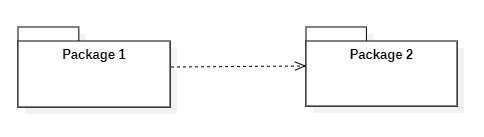
\includegraphics{../immagini/normeUML/pk_uml.png}
		\caption{Rappresentazione grafica dei diagrammi dei package}
\end{figure}
\paragraph{Diagrammi delle classi:}\label{ProcessiPrimariProgettazioneUMLDiagrammiDelleClassi}
Le classi vengono individuate da un rettangolo suddiviso in tre sezioni orizzontali. Ciascuna sezione partendo dall'alto individuano:
\begin{enumerate}
	\item \textbf{Nome della classe}: deve essere univoco ed esplicativo. Il nome sarà scritto in lingua inglese, se la classe raffigurata è una classe astratta il suo nome verrà preceduto da $<<abstract>>$, mentre se è un'interfaccia verrà preceduto da $<<interface>>$.
	\item \textbf{Attributi}: ogni attributo individua una variabile della classe. Gli attributi vengono scritti uno dopo l'altro sotto forma di lista. Ogni attributo sarà scritto nel seguente modo:
	\begin{center}
		\textbf{nomeAttributo : tipo}
	\end{center}
	La descrizione della scrittura degli attributi è la seguente:
	\begin{itemize}
		\item \textbf{nomeAttributo}: individua il nome della variabile, deve essere scritta in lingua inglese e con la lettera iniziale minuscola. Nel caso sia una variabile costante tutto il nome deve essere scritto in maiuscolo;
		\item \textbf{tipo}: il tipo può essere semplice o definito da una classe creata dall'utente.
	\end{itemize}
	Ogni attributo viene preceduto obbligatoriamente da un operatore:
	\begin{itemize}
		\item \textbf{$+$}: indica la visibilità pubblica della variabile;
		\item \textbf{$-$}: indica la visibilità privata della variabile;
		\item \textbf{$\#$}: indica la visibilità protetta della variabile;
		\item \textbf{$\thicksim$}: indica la visibilità package della variabile.
	\end{itemize}
	\item \textbf{Metodi}: indicano i metodi della classe, vengono disposti in lista uno dopo l'altro. I metodi vengono scritti nel seguente modo:
	\begin{center}
		\textbf{nomeMetodo (lista-param) : tipoR}
	\end{center}
	La descrizione della scrittura dei metodi è la seguente:
	\begin{itemize}
		\item \textbf{nomeMetodo}: individua il nome del metodo, deve essere univoco ed in lingua inglese;
		\item \textbf{lista-param}: indica la lista dei parametri formali del metodo che può essere composta da 0 o più parametri, ogni parametro è separato da una virgola con il successivo e sono scritti nel formato \textit{nome : tipo};
		\item \textbf{tipoR}: individua il tipo dell'oggetto di ritorno, può essere semplice o definito dall'utente.
	\end{itemize}
	Ogni metodo sarà preceduto dagli operatori di visibilità descritti precedentemente. Se il metodo sotto osservazione è un metodo astratto il suo nome viene preceduto da $<<abstract>>$, mentre se è statico da $<<static>>$.
\end{enumerate}
Il collegamento tra i diagrammi delle classi viene effettuato con delle frecce che illustrano le dipendenze.
I tipi di frecca vengono descritti di seguito:
\begin{itemize}
	\item freccia normale, da classe 1 a classe 2: indica che gli oggetti delle due classi consividono una relazione statica;
	\begin{figure}[H]
		\centering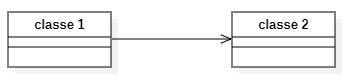
\includegraphics{../immagini/normeUML/frecSempl.png}
		\caption{Relazione di associazione tra classe 1 e classe 2}
	\end{figure}

	\item freccia tratteggiata, da classe 1 a classe 2: indica che la definizione di una delle due classi fa riferimento alla definizione dell'altra;
	\begin{figure}[H]
		\centering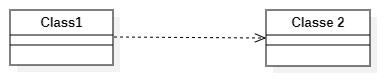
\includegraphics{../immagini/normeUML/frecTrat.png}
		\caption{Relazione di dipendenza tra classe 1 e classe 2}
	\end{figure}
	\item freccia "a diamante" vuoto, da classe 1 a classe 2: indica una relazione del tipo "è parte di", cioè classe 2 è parte di classe 1, questo permette di aggregare più classi e creare una classe più complessa;
	\begin{figure}[H]
		\centering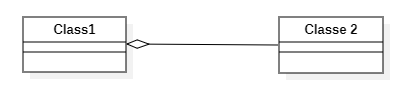
\includegraphics{../immagini/normeUML/frecDiamVuot.png}
		\caption{Relazione di aggregazione tra classe 1 e classe 2}
	\end{figure}
	\item freccia "a diamante" piena, da classe 1 a classe 2: indica la composizione, è simile all'aggregazione, ma ha una relazione più forte sulla classe sub-ordinata perchè classe 2 non può esistere la classe 1;
	\begin{figure}[H]
		\centering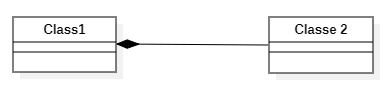
\includegraphics{../immagini/normeUML/frecDiamPien.png}
		\caption{Relazione di composizione tra classe 1 e classe 2}
	\end{figure}
	\item freccia con punta vuota, da classe 1 a classe 2: indica la realizzazione/implementazione, cioè l'oggetto classe 1 implementa il comportamento, quindi nel nostro caso i metodi, che l'oggetto classe 2 specifica.
	\begin{figure}[H]
		\centering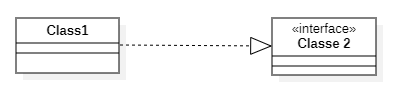
\includegraphics{../immagini/normeUML/frecInter.png}
		\caption{Relazione di interfaccie tra classe 1 e classe 2}
	\end{figure}
\end{itemize}
Ad ogni freccia di collegamento viene indicato la molteplicità che ha e vengono indicate nel seguente modo:
\begin{itemize}
	\item \textbf{1}: classe 1 possiede un'istanza di classe 2;
	\item \textbf{0...1}: classe 1 può possedere al massimo una istanza di classe 2;
	\item \textbf{0...*} classe 1 può possedere 0 o più istanze della classe 2;
	\item \textbf{*}: classe 1 può possedere più istanze della classe 2;
	\item \textbf{n}: classe 1 possiede $n$ istanze della classe 2.
\end{itemize}
\paragraph{Diagrammi delle attività:}\label{ProcessiPrimariProgettazioneUMLDiagrammiDellAttività}
Il diagramma di attività è un tipo di diagramma che permette di descrivere un processo attraverso dei grafi in cui i nodi rappresentano le attività e gli archi l'ordine con cui vengono eseguite. I diagrammi vengono illustrati usando il seguente formalismo:
\begin{itemize}
	\item \textbf{Nodo iniziale}: viene rappresentato da un pallino nero pieno ed indica l'inizio della attività dove viene generato un token;
	\begin{figure}[H]
		\centering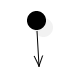
\includegraphics{../immagini/normeUML/nodoIni.png}
		\caption{Rappresentazione di un nodo iniziale}
	\end{figure}
	\item \textbf{Attività}: viene rappresentata da un rettangolo, la sua descrizione deve essere breve e significativa per indicare l'azione svolta in quel punto del flusso dell'attività. Consuma e produce un token;
	\begin{figure}[H]
		\centering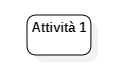
\includegraphics{../immagini/normeUML/attivita.png}
		\caption{Rappresentazione di una attività}
	\end{figure}
	\item \textbf{Nodo finale}: viene rappresentato da due cerchi concentrici di cui l'esterno è vuoto e quello interno è pieno. Indica il punto in cui termina l'esecuzione. Consuma un token;
	\begin{figure}[H]
		\centering
\includegraphics{../immagini/normeUML/nodoFine.png}
		\caption{Rappresentazione di un nodo finale}
	\end{figure}
	\item \textbf{Nodo di fine flusso}: viene rappresentato attraverso un cerchio vuoto con una $X$ al centro. Indica la terminazione di un ramo dell'attività. Consuma un token;
	\begin{figure}[H]
		\centering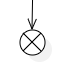
\includegraphics{../immagini/normeUML/nodoFineFlusso.png}
		\caption{Rappresentazione di un nodo di fine flusso}
	\end{figure}
	\item \textbf{Sotto-attività}: viene rappresentata da un rettangolo con un tridente nell'angolo in basso a destra. Indica che l'attività viene rappresentata in un diagramma separato ed ogni sotto-attività ha un input ed un output;
	\begin{figure}[H]
		\centering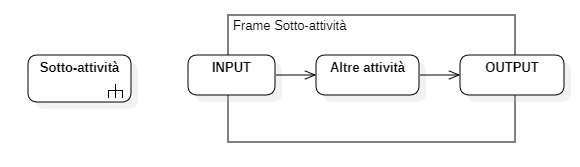
\includegraphics{../immagini/normeUML/attSott.png}
		\caption{Rappresentazione di una sotto-attività}
	\end{figure}
	\item \textbf{Branch}: viene rappresentato attraverso un rombo con una freccia in entrata e $n$ frecce in uscita. Ogni ramo in uscita deve avere una guardia, scritta nel formato $[guardia]$. Il branch definisce una scelta, tra i rami disponibili in usciti se ne può scegliere uno solo in base alla guardia. Consuma e produce un token;
	\item \textbf{Merge}: viene rappresentato da un rombo con $n$ frecce in entrata e una freccia in uscita. Individua il punto in cui i rami creati dal Branch tornano ad unirsi. Consuma e produce un token;
		\begin{figure}[H]
		\centering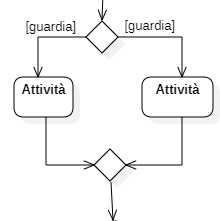
\includegraphics{../immagini/normeUML/mergeBranch.png}
		\caption{Rappresentazione di un branch e merge}
	\end{figure}
	\item \textbf{Fork}: viene rappresentato da una linea nera marcata orizzontale o verticale. Indica il punto in cui avviene una paralizzazione delle attività da effettuare senza un limite temporale. Il fork presenta una freccia in entrata e $n$ frecce in uscita. Consuma e produce un token;
	\item \textbf{Join}: viene rappresentato da una linea nera marcata orizzontale o verticale. Indica il punto in cui tutte le attività svolte in parallelo si sincronizzano. Il join preseta $n$ frecce in entrata e una freccia in uscita. Consuma e produce un token;
		\begin{figure}[H]
		\centering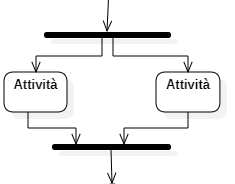
\includegraphics{../immagini/normeUML/forkJoin.png}
		\caption{Rappresentazione di un fork e un join}
	\end{figure}
	\item \textbf{Pin}: viene rappresentato da un quadrato con una freccia al suo interno nella direzione di input o output. Indica il parametro che viene inviato da un'attività all'altra, a fianco del quadrato viene scritto il tipo di parametro inviato;
		\begin{figure}[H]
		\centering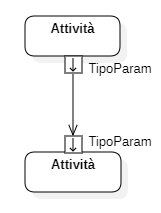
\includegraphics{../immagini/normeUML/pin.png}
		\caption{Rappresentazione di pin in un'attività}
	\end{figure}
	\item \textbf{Segnali}: rappresentate da due figure "a incastro", la prima utilizzata per l'emissione del segnale, la seconda per la ricezione dello stesso. Il testo di descrizione all'interno delle figure deve essere breve e conciso e deve avere un prefisso $-signal sending-$ o $-signal receipt-$ a secondo della figura in descrizione;
		\begin{figure}[H]
		\centering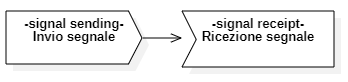
\includegraphics{../immagini/normeUML/signal.png}
		\caption{Rappresentazione di un segnale}
	\end{figure}
	\item \textbf{Timeout}: viene rappresentato da una clessidra stilizzata. Indica due tipi di eventi uno è il timeout rappresentato dalla clessidra con una freccia entrante e uscente, serve a rappresentare un'attesa di tempo. L'altro tipo di evento è l'evento ripetuto, rappresentato da una clessidra con una freccia in uscita, serve ad indicare un'azione ripetuta. %??? immagini%
		\begin{figure}[H]
		\centering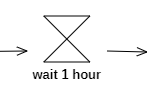
\includegraphics{../immagini/normeUML/timeout.png}
		\centering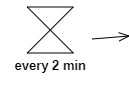
\includegraphics{../immagini/normeUML/reapeate.png}
		\caption{Rappresentazione di un evento timeout e uno ripetuto}
	\end{figure}
\end{itemize}

\paragraph{Diagrammi dei casi d'uso:}\label{ProcessiPrimariProgettazioneUMLDiagrammiCasiUso}
I diagrammi di dei casi d'uso descrivono le funzionalità del sistema attraverso una visione esterna. Nello specifico, un caso d'uso è un'insieme di scenari e sequenze di azioni che hanno lo stesso obiettivo per l'utente. Un diagramma non deve rappresentare alcun dettaglio implementativo, permettendo una descrizione delle funzionalità coinvolte con una visione esterna al sistema, come se fosse percepita dall'utente. Gli elementi presenti all'interno di un caso d'uso sono i seguenti:
\begin{itemize}
	\item \textbf{Attore:} viene disegnato come un omino stilizzato e sotto viene posto il nome;
	\item \textbf{Caso d'uso:} rappresentato con un ovale e al suo interno viene inserita la descrizione dello stesso. Ogni caso d'uso viene associato ad un attore e viceversa per mezzo di una linea semplice;	
\end{itemize}
Gli elementi contenuti all'interno di un diagramma in base alle funzionalità che devono essere rappresentate, le seguenti relazioni:
\begin{itemize}
\item \textbf{Associazione:} è la comunicazione diretta tra attore ed use case. Rappresenta la partecipazione dell'attore al caso d'uso a cui è collegato. Un'associazione viene rappresentata mediante una linea che collega l'attore al caso d'uso;
\item \textbf{Inclusione:} L'inclusione è un legame diretto stretto tra due use case. Dati due casi d'uso A e B, si dice che A include B se ogni istanza di A esegue B. B è incluso nell'esecuzione di A e la responsabilità di esecuzione di B è unicamente di A. Un'inclusione viene rappresentata con una freccia tratteggiata, che collega i casi d'uso coinvolti, in direzione del caso d'uso incluso;
\item \textbf{Estensione:} L'estensione aumenta le funzionalità di uno use case. Dati due casi d'uso A e B, si dice che B estende A se A esegue B solo a determinate condizioni. L'esecuzione di B interrompe A e per questo motivo viene utilizzata prevalentemente per gestire errori ed eccezzioni. Un'estensione viene rappresentata con una freccia tratteggiata, che collega i casi d'uso coinvolti, dal caso d'uso che estende a quello che viene esteso, e un quadrato con l'angolo in alto a destra piegato, contenente le condizioni necessarie per il verificarsi dell'estensione e il nome della stessa;
\item \textbf{Generalizzazione:} La generalizzazione è un legame tra attori o più raramente tra use case. Dati due casi d'uso A e B, A è generalizzata di B se condivide almeno le funzionalità di A. B può modificare le funzionalità di A, mentre tutte le funzionalità non ridefinite si mantengono identiche a quelle di A. Le generalizzazioni vengono rappresentate con una freccia continua vuota dall'elemento figlio all'elemento padre.
\end{itemize}


\paragraph{Diagrammi di sequenza:}\label{ProcessiPrimariProgettazioneUMLDiagrammiDiSequenza}
I diagrammi di sequenza rappresentano dettagliatamente come gli oggetti interagiscono tra di loro tramite messaggi. Ogni entità del diagramma è collegata mediante una linea tratteggiata ad un'altra entità con lo stesso contenuto. Tale linea indica il passare del tempo. Le entità del diagramma si scambiano messaggi sotto forma di frecce che assumono una diversa struttura a seconda del tipo di messaggio che si sta inviando. \\
I costrutti utilizzati in questi diagrammi sono i seguenti:

\begin{itemize}
	\item \textbf{partecipante}: rappresenta un oggetto che detiene il flusso di esecuzione e collabora alla realizzazione di un comportamento. \\
	Il partecipante è così composto:
\begin{itemize}
	\item \textbf{nome}: nome dell'oggetto partecipante;
	\item \textbf{barra di attivazione}: indica la durata del periodo di tempo durante il quale il partecipante è attivo;
\end{itemize}
	\item \textbf{messaggio}: rappresenta un'operazione di un partecipante che viene chiamata da parte di un altro partecipante e i dati scambiati tra i due.\\
	Un messaggio può essere:
\begin{itemize}
	\item \textbf{sincorno}: messaggio di chiamata in cui il partecipante chiamante attende la risposta del partecipante chiamato prima di proseguire la sua esecuzione. Viene utilizzata una freccia piena e sopra tale freccia va specificato il metodo invocato;
	\item \textbf{asincrono}: messaggio di chiamata in cui il partecipante chiamante non attende la risposta del partecipante chiamato, ma prosegue la sua esecuzione subito dopo la chiamata. Viene utilizzata una freccia e sopra tale freccia va specificato il metodo invocato;
	\item \textbf{ritorno}: messaggio di ritorno riferito ad un precedente messaggio di chiamata. Viene utilizzata una freccia tratteggiata e sopra tale freccia va indicato il tipo di ritorno;
	\item \textbf{creazione}: messaggio di creazione di un nuovo partecipante da parte del partecipante chiamante. Viene utilizzata una freccia tratteggiata accompagnata dalla parola $<<create>>$;
	\item \textbf{distruzione}: messaggio di distruzione di un partecipante da parte del partecipante chiamante. Viene utilizzata una freccia piena accompagnata dalla parola $<<destroy>>$.
\end{itemize}
	\item \textbf{frame di interazione}: rappresenta un ciclo o una condizione che coinvolge più messaggi e parti delle barre di attivazione di più partecipanti. \\
	Un frame è caratterizzato dalle proprietà di:
\begin{itemize}
	\item \textbf{guardia}: indica la condizione di attivazione del frame, posta in corrispondenza del partecipante coinvolto;
	\item \textbf{etichetta}: indica la tipologia del frame.
\end{itemize}
\end{itemize}
Esistono diverse etichette per identificare i frame d'interazione. I progettisti dovranno attenersi alle seguenti:
\begin{itemize}
	\item \textbf{alt}: alternativa (tra più frame), è seguito solo il frame per cui la guardia è verificata;
	\item \textbf{opt}: opzionale, il frame è eseguito solo se la guardia è verificata;
	\item \textbf{par}: parallelo, ogni frame è eseguito in parallelo;
	\item \textbf{loop}: ciclo, il frame può essere eseguito più volte, in base al verificarsi della guardia;
	\item \textbf{region}: regione critica, il frame può essere eseguito da un solo flusso di esecuzione alla volta;
	\item \textbf{neg}: negativo, il frame rappresenta un'iterazione non valida;
	\item \textbf{ref}: riferimento, il frame si riferisce ad un'iterazione definita in un'altro diagramma;
	\item \textbf{sd}: diagramma di sequenza, il frame comprende un intero diagramma di sequenza.
\end{itemize}
\subsection{Codifica}\label{ProcessiPrimariCodifica}

\subsubsection{Scopo}\label{ProcessiPrimariCodificaScopo}
La fase di codifica è la scrittura del codice per sviluppare la miglior soluzione del prodotto. In questa sezione si introdurranno tutte le norme necessarie allo sviluppo di un codice uniformato tra tutti i \textit{Programmatori} e rispettoso delle regole standard indicate nel documento.

\subsubsection{Descrizione}\label{ProcessiPrimariCodificaDescrizione}
In questa fase la programmazione del prodotto dovrà rispettare le norme descritte nel documento. Perseguendo gli obiettivi individuati nel documento \textit{Piano di qualifica 2.0.0} si produrrà un software con un'alta qualità di codice.

\subsubsection{Aspettative}\label{ProcessiPrimariCodificaAspettative}
Conclusa la fase di codifica ci si attende un codice pulito e facile da leggere, utile nelle successive validazioni, modifiche e per agevolare la sua manutenzione. L'obiettivo è quello di sviluppare un prodotto conforme alle richieste individuate con il proponente$_{\scaleto{G}{3pt}}$.

\subsubsection{Intestazione} \label{ProcessiPrimariCodificaIntestazione}
Ciascun file di codifica dovrà riportare la seguente intestazione:
\begin{center}
	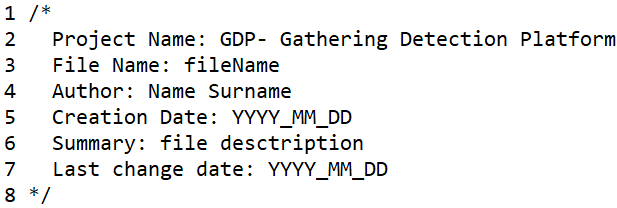
\includegraphics[width=0.5\linewidth]{../immagini/IntestazioneNorme.png}
\end{center}

\subsubsection{Stile di codifica}\label{ProcessiPrimariCodificaStileDiCodifica}
All'interno di questo paragrafo vengono elencate le norme da rispettare da ogni membro del gruppo per raggiungere uniformità del codice:

\begin{itemize}
	\item \textbf{Indentazione}: ogni blocco di codice scritto per il prodotto da sviluppare deve essere ben indentato e deve rispettare per ciascun livello una misura di 4 spazi. E’ obbligatorio utilizzare gli spazi anzichè le tabulazioni (tasto tab). Per riuscire a rispettare tale obbligo si cosiglia di configurare in modo appropriato il proprio editor o IDE. Fanno eccezione a queste regole i commenti che vengono inseriti per spiegazioni di blocchi di codice;
	\item \textbf{Parentesizzazione}:  le parentesi devono essere utilizzate in linea col blocco di codice scritto e non in una linea sottostante, separandole con un singolo spazio;
	\item \textbf{Univocità delle classi, variabili, metodi e funzioni}: ogni classe, variabile, metodo e funzione utilizzata deve avere un nome significativo, esplicativo ed univoco;
	\item \textbf{Classi}: ogni classe deve avere il proprio nome scritto con l'iniziale maiuscola;
	\item \textbf{Metodi e funzioni}: il nome di metodi e funzioni devono iniziare per lettera minuscola e se composti da più parole le successive devono essere scritte con lettera maiuscola (stile \textit{CamelCase});
	\item \textbf{Commenti}: i commenti vanno inseriti solo nei casi in cui sono necessari per migliorare la comprensibilità e leggibilità del codice, mantenendo uno stile sintetico. Si possono utilizzare due tipologie di costrutti per i commenti:
	\begin{itemize}
		\item \textbf{/* ... */} per i commenti che racchiudono più di una riga, lasciare la riga vuota dopo la dicitura /* ed andare a capo per descrivere una parte di codice e poi chiudere il commento con la dicitura */ nella riga successiva alla descrizione;
		\item \textbf{// … } per i commenti di linea singola che devono essere separati da uno spazio dopo la dicitura //.
	\end{itemize}
	Questa dicitura legata ai commenti non è valida per il linguaggio Python$_G$ in quanto al loro posto si usa il cancelletto {\symbol{35}}.
	Il commento verrà scritto in linea al simbolo appena illustrato.
	I costrutti non devono essere riportati sulla stessa riga dell’istruzione a cui si riferiscono ma sulla riga che la precede;
	\item \textbf{Lingua}: il codice ed i commenti devono essere scritti in lingua inglese.
\end{itemize}

\subsubsection{Python}\label{ProcessiPrimariCodificaPython}
Si tratta di un linguaggio di programmazione definito "ad alto livello" rispetto alla maggior parte di essi.
Si tratta di un linguaggio orientato ad oggetti, utile a sviluppare script, computazione numerica e sviluppare software.
Nel progetto \textit{Gathering-Detection-Platform}, Python$_G$ è il linguaggio su cui si basa il modulo Prediction e Acquisition.

\begin{itemize}
	\item versione utilizzata: 3.8.x;
	\item link download: \url{https://www.python.org/downloads/} .
\end{itemize}

\subsubsection{Java}\label{ProcessiPrimariCodificaJava}
Si tratta di una piattaforma che ha come caratteristica principale il fatto di rendere possibile scrittura ed esecuzione di applicazioni indipendenti dall'hardware di esecuzione.
Il risultato è una virtualizzazione dalla piattaforma stessa, che rende così il linguaggio Java$_{\scaleto{G}{3pt}}$, e i relativi programmi, portabili su piattaforme hardware diverse. Questo linguaggio viene utilizzato per la codifica del applicativo con framework Spring$_{\scaleto{G}{3pt}}$ del modulo back-end$_{\scaleto{G}{3pt}}$ della web-app$_{\scaleto{G}{3pt}}$.

\begin{itemize}
	\item versione utilizzata: 11.x;
	\item link download: \url{https://www.java.com/it/download/}.
\end{itemize}

\subsubsection{HTML}\label{ProcessiPrimariCodificaHTML}
HTML$_G$, acronimo di HyperText Markup Language, è un linguaggio di mark up per siti web.
Era stato ideato per la formattazione e impaginazione di pagine ipertestuali sul web.
Oggi giorno viene utilizzato soprattutto per gestire la separazione tra la struttura logica della pagina web e la sua rappresentazione, gestita dal CSS$_G$.
Nel progetto questo linguaggio viene utilizzato per sviluppare la parte di web-app${\scaleto{G}{3pt}}$, interagendo con anche JavaScript${\scaleto{G}{3pt}}$, CSS${\scaleto{G}{3pt}}$, Bootstrap$_G$ e Vue.js$_G$.

\subsubsection{CSS}\label{ProcessiPrimariCodificaCSS}
Il CSS$_{\scaleto{G}{3pt}}$ è il principale linguaggio utilizzato per definire la formattazione dei siti e pagine web.
L'utilizzo del CSS${\scaleto{G}{3pt}}$ permette di separare i contenuti della pagina HTML${\scaleto{G}{3pt}}$ dal proprio layout ma anche di rendere la programmazione più chiara e facile da utilizzare, garantendo il riutilizzo di codice e facilitando la manutenzione.
Nel progetto viene utilizzato per formattare il layout estetico della web-app${\scaleto{G}{3pt}}$.

\subsubsection{Vue.js}\label{ProcessiPrimariCodificaVue}
È un framework JavaScript$_G$, utilizzato per la creazione di interfacce utente e applicazione single-page.
Supporta molte funzionalità, anche avanzate, grazie ad una serie di librerie di supporto dedicate che sono ufficialmente mantenute.

\begin{itemize}
	\item versione utilizzata: 2.6.12;
	\item link al sito: \url{https://vuejs.org/}.
\end{itemize}

\subsection{Strumenti}\label{ProcessiPrimariStrumenti}

\subsubsection{PragmaDB}\label{ProcessiPrimariStrumentiPragmaDB}
Programma utilizzato per il tracciamento dei requisiti$_{\scaleto{G}{3pt}}$.
\begin{center}
	\url{https://pragmadb.com/}
\end{center}
\subsubsection{StarUML}\label{ProcessiPrimariStrumentiDrawIo}
Questo strumento viene usato per la realizzazione di diagrammi UML$_{\scaleto{G}{3pt}}$ in quanto è stato ritenuto semplice da utilizzare.
\begin{center}
	\url{https://staruml.io/}
\end{center}
\subsubsection{Atom}\label{ProcessiPrimariStrumentiAtom}
IDE che viene usato per la codifica del linguaggio Java$_G$ e Javascript$_G$, oltre a supportare anche altri molteplici linguaggi di programmazione come Python$_{\scaleto{G}{3pt}}$, C, C++ e anche \LaTeX. Offre la piena compatibilità con Linux, Windows, macOS e fornisce molte integrazioni aggiuntive.
\begin{center}
	\url{https://atom.io}
\end{center}
\subsubsection{PyCharm}\label{ProcessiPrimariStrumentiPyCharm}
Si tratta di un IDE per programmare con il linguaggio Python$_{\scaleto{G}{3pt}}$.
Offre molteplici plugin.
\begin{center}
	\url{https://www.jetbrains.com/pycharm/}
\end{center}
\subsubsection{Google.Colab}\label{ProcessiPrimariStrumentiGoogleColab}
Colab, diminutivo di Colaboratory, è uno strumento online offerto da Google.
Mette a disposizione l'hardware di Google in modo da permettere a chiunque di poter testare script o modelli pesanti (es. Machine Learning$_{\scaleto{G}{3pt}}$) nel caso la propria macchina non ne fosse in grado.
Non prevede alcuna configurazione da parte dell'utente.
\begin{center}
	\url{https://colab.research.google.com/notebooks/}
\end{center}
\subsubsection{LeafLet}\label{ProcessiPrimariStrumentiLeafLet}
Utilizzato per la realizzazione delle Heat-map.
Si tratta di una libreria Open-Source basato su Javascript$_{\scaleto{G}{3pt}}$.
\begin{center}
	\url{https://leafletjs.com/}
\end{center}
\subsubsection{Maven} \label{ProcessiPrimariStrumentiMaven}
	Maven$_G$ è uno strumento di build automation$_G$, sviluppato da \textit{Apache}, utilizzato per la gestione di progetti Java$_{\scaleto{G}{3pt}}$. Maven$_{\scaleto{G}{3pt}}$ si basa sul concetto di \textit{Project Object Model} (POM), ovvero un file .xml in cui sono specificate le informazioni e configurazioni necessarie allo sviluppo di un'applicazione Java. Maven$_{\scaleto{G}{3pt}}$, infatti, permette di configurare tutte le dipendenze ed i plugin, specificati nel pom.xml, autonomamente.
	\begin{center}
		\url{https://maven.apache.org/}
	\end{center}
\subsubsection{PostMan}\label{ProcessiPrimariStrumentiPostMan}
È un’applicazione che consente di costruire, testare e documentare API più velocemente. Nel nostro caso è stato utilizzato per testare la connessione e il funzionamento dei servizi creati nell'applicativo di Spring.
\begin{center}
	\url{https://www.postman.com/}
\end{center}
\subsubsection{Jupyter Notebook}\label{ProcessiPrimariStrumentiJupyterNotebook}
Si tratta di un’applicazione web open-source$_{\scaleto{G}{3pt}}$ che ti permette di creare e condividere documenti che contengono codice, equazioni, visualizzazioni e testo narrativo, è particolarmente indicato per la pulizia dei dati e la loro trasformazione per l’utilizzo per il machine learning$_{\scaleto{G}{3pt}}$.
\begin{center}
	\url{https://jupyter.org/index.html/}
\end{center}
\subsubsection{Anaconda}\label{ProcessiPrimariStrumentiAnaconda}
Ambiente di distribuzione Python$_{\scaleto{G}{3pt}}$ che raccoglie molti pacchetti open source$_{\scaleto{G}{3pt}}$ e facili da installare, il vantaggio di usare questo strumento è la semplicità con cui si può creare il proprio ambiente di sviluppo virtuale.
\begin{center}
	\url{https://www.anaconda.com/}
\end{center}

